\chapter{Development of a device for direct counting of the number of particles in the beam}

\section{Introduction}
This chapter will focus on the devices used within the MoVe\_IT project in order to obtain a single proton counting device.
This comprehends the solid state detector, the ASICs used to digitalise the signal and the board final read-out board.
\begin{figure}[H]
	\centering
	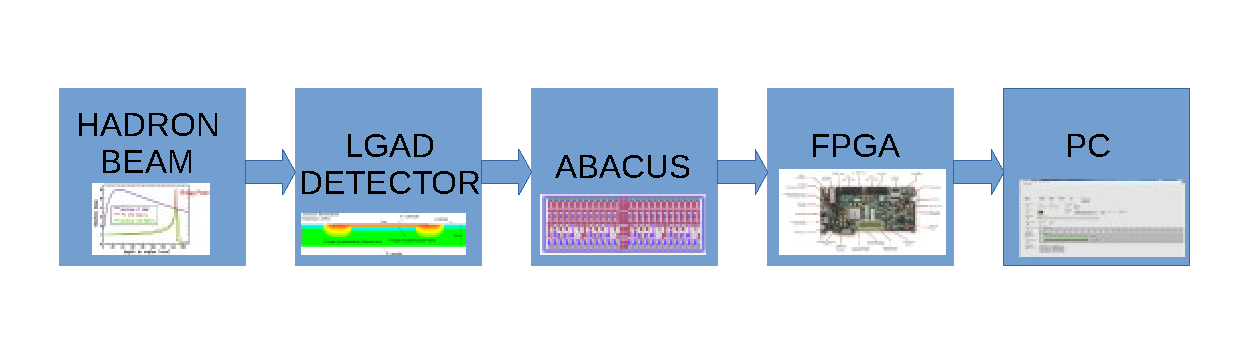
\includegraphics[width=0.99\linewidth]{IMG/ch2/BLOCK}
	\caption{Data flow, from beam to pc}
	\label{fig:block}
\end{figure}
\noindent In figure \ref{fig:block} it can be seen a diagram with the "data flow" of the Project.
The particle beam coming from the accelerators are detected by a LGAD sensor that will be discussed in section \ref{lgad}, the current signal coming from the detector is the digitalized by the second version of a full custom circuit called ABACUS\_v2 that will be discussed in section \ref{chip}.
This ASIC will be mounted on a full custom PCB that will be analysed in section \ref{esaabacus}.
The data from the chip is read by a FPGA board, a general purpose device that will be analysed in detail within chapter 4.
The FPGA elaborates the data and finally sends them to a computer.  

\section{Low Gain Avalanche Diode (LGAD)}\label{lgad}
\cite{lgad}
\begin{figure}[H]
	\centering
	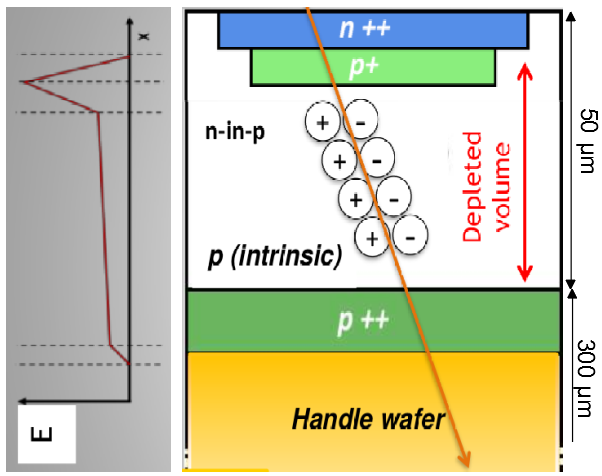
\includegraphics[width=0.35\linewidth]{IMG/ch2/UFSDLGAD.png}
	\caption{LGAD detector diagram}
	\label{fig:ufsdlgad}
\end{figure}

\section{ABACUS chip}\label{chip}
\begin{figure}[H]
	\centering
	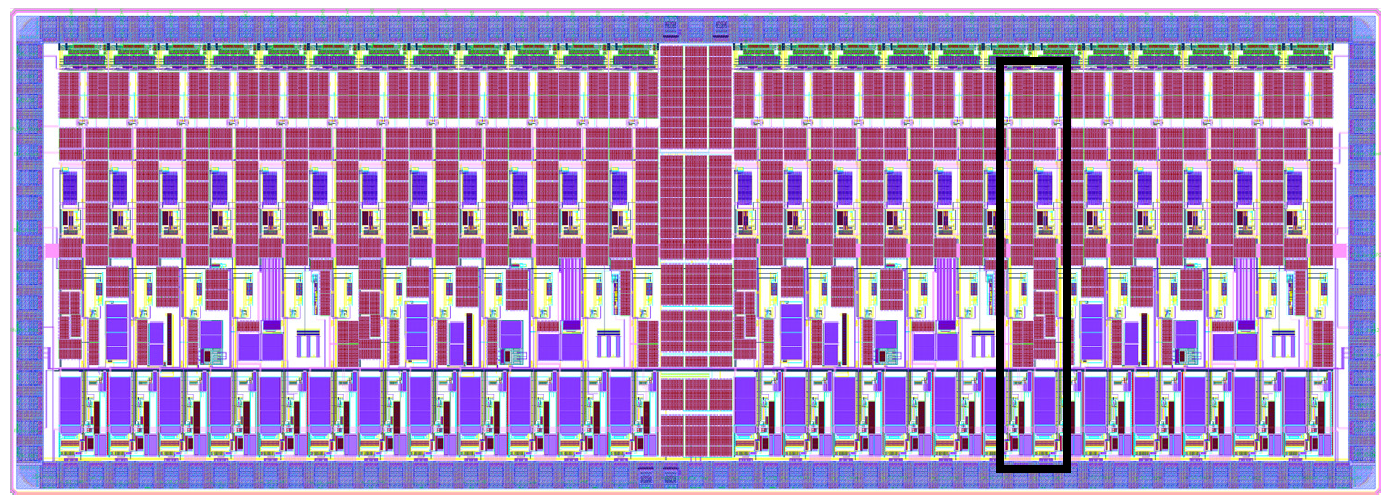
\includegraphics[width=0.9\linewidth]{IMG/ch2/ABACUS2.png}
	\caption{ABACUS\_v2 chip die view}
	\label{fig:abacus2}
\end{figure}

\begin{figure}[H]
	\centering
	\includegraphics[width=0.8\linewidth]{IMG/ch2/Abacus_channel.png}
	\caption{Single channel diagram of the ABACUS\_v2 chip}
	\label{fig:abacuschannel}
\end{figure}

\section{Esa-Abacus}\label{esaabacus}
\begin{figure}[H]
	\centering
	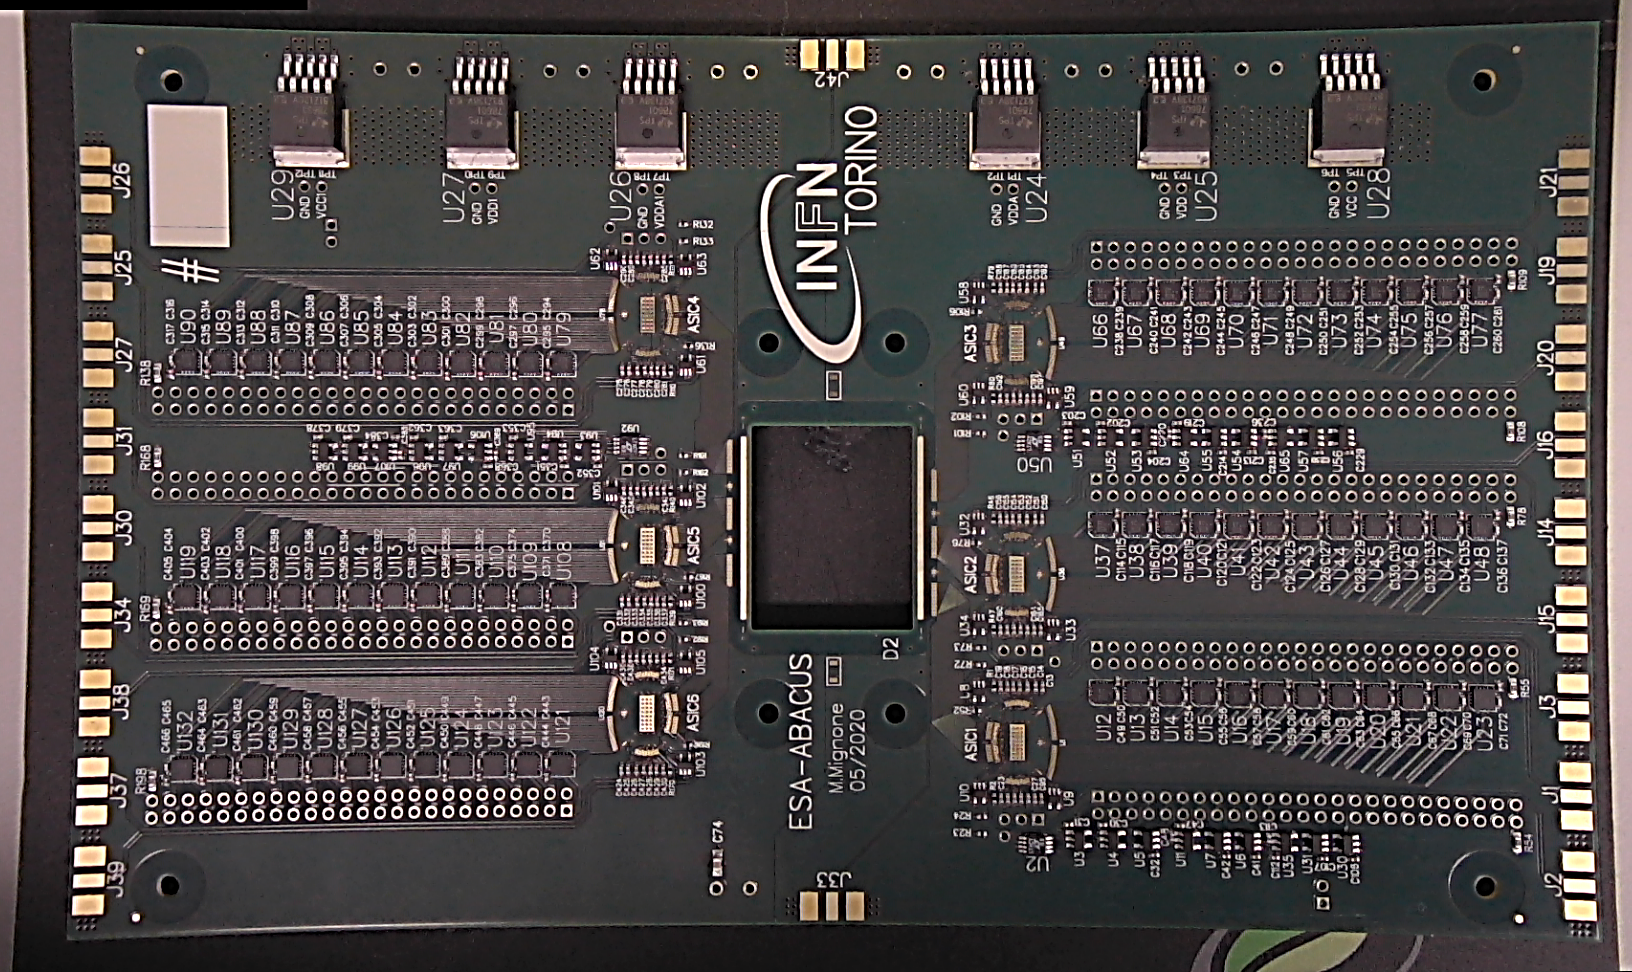
\includegraphics[width=0.7\linewidth]{IMG/ch2/EsaAbacus.png}
	\caption{Esa-Abacus board}
	\label{fig:esaabacus}
\end{figure}

\section{FPGA board}

%\section{Beam test with strip sensor}
%\section{Verification of counting skills}